%----------------------------------------------------------------------------------------
%	PACKAGES AND DOCUMENT CONFIGURATIONS
%----------------------------------------------------------------------------------------

\documentclass{article}


\usepackage{graphicx} % Required for the inclusion of images
\graphicspath{{figures/}}
\usepackage{subfigure} % Required for the inclusion of images
\usepackage{natbib} % Required to change bibliography style to APA
\usepackage{amsmath} % Required for some math elements 
\usepackage{listings}
\usepackage{xcolor}
\usepackage{fontspec}
\usepackage{ctex}
\usepackage{geometry}
\geometry{a4paper,scale=0.8}
\renewcommand{\contentsname}{\centerline{目录}}
\setmonofont{Consolas}
\lstset{
basicstyle=\ttfamily\footnotesize,%
escapeinside=``,%
keywordstyle=\color{black},%\bfseries, \underbar,%
identifierstyle={},%
tabsize=4,
commentstyle=\color{blue},%
stringstyle=\ttfamily,%
%labelstyle=\tiny,%
extendedchars=false,%
linewidth=\textwidth,%
numbers=left,%
numberstyle=\tiny \color{blue},%
frame=trbl%
}
%点列
%\begin{itemize}
%\item[$\bullet$]Get familiar with Y86 assembly language.
%\end{itemize}

%小标题
%\begin{center}
%{\ttfamily rsum.ys}
%\end{center}
%代码
%\begin{lstlisting}[language={[ANSI]C}]
%\end{lstlisting}
%点列和浮动体图表和ref
%\begin{itemize}
%\item[$\bullet$]{\ttfamily sum.ys} (Figure \ref{Part A: sum.ys})\\
%\end{itemize}
%\begin{figure}[htbp]%figure浮动体环境 [htbp]指定位置
%		\centering%居中排版
%		\includegraphics{A_sum}
%		\caption{Part A  {\ttfamily sum.ys}} \label{Part A: sum.ys}%标题 自动编号 label标签
%\end{figure}


%\usepackage{times} % Uncomment to use the Times New Roman font

%----------------------------------------------------------------------------------------
%	DOCUMENT INFORMATION
%----------------------------------------------------------------------------------------

\title{\textbf{操作系统课程设计Project 8\\Designing a Virtual Memory Manager}} % Title

\author{姓名: 郭倩昀  
\\班级: F1903303  
\\学号: 519021910095  
\\Email: guoqianyun@sjtu.edu.cn} % Author name and email
\date{\today} % Date for the report
\begin{document}
\maketitle % Insert the title, author and date
\tableofcontents
\newpage
\section{Designing a Virtual Memory Manager}
\subsection{实验内容与目标}
本实验需要利用C语言设计虚拟内存管理系统,使得可以根据逻辑地址正确读取数据并正确管护物理内存,页表,TLB,主要可以分为一下几个部分。
\begin{itemize}
\item[$\bullet$]管理物理内存
\item[$\bullet$]管理TLB
\item[$\bullet$]管理页表
\end{itemize}
\subsection{实验过程及步骤}
\begin{itemize}
\item[$\bullet$]定义基本参数\\
根据书本指示定义页面数,页面大小,TLB大小,内存帧数和内存帧大小。其中内存帧数与页面数相等为256时不需要页面替换算法,但是如果设计内存帧数为128,则需要设计页面替换算法,这里选择使用LRU置换策略进行页面替换。
\item[$\bullet$]管理物理内存\\
管理物理内存需要支持的操作有维护空闲帧列表,初始化物理内存(包括初始化空闲帧列表),将一个页面调入物理内存(如果无空闲帧,则要用LRU算法选取替换帧替换),根据帧数和offset访问物理内存,清空内存等操作。为了支持LRU页面置换算法,需要维护帧的LRU信息,每次访问都要更新LRU信息。
\begin{itemize}
\item[$\bullet$]维护空闲帧列表主要用init\_empty\_frame\_list函数初始化空闲帧列表(插入内存帧数的空闲帧列表),get\_empty\_frame函数从空闲帧列表中找出一个空闲帧返回frame num(未找到则返回-1),clean\_empty\_frame\_list函数释放所有的空闲帧。
\item[$\bullet$]初始化物理内存使用init\_memory函数,打开后备存储,调用init\_empty\_frame\_list初始化内存帧,同时为了支持LRU置换,初始化帧的LRU信息。
\item[$\bullet$]将一个页面调入物理内存使用add\_page\_into\_memory函数,先根据page number读取后备存储的数据,寻找一个空闲帧,(若未找到则通过LRU置换一个帧,置换出的帧需要修改页表的有效-无效位),将数据放入空闲帧并更新LRU信息,返回frame number。
\item[$\bullet$]问物理内存使用access\_memory函数根据帧数和offset访直接读取,但要更新LRU信息。
\item[$\bullet$]清空内存使用clean\_memory函数,调用clean\_empty\_frame\_list函数释放所有的空闲帧并关闭打开的后备存储文件。
\end{itemize}
\item[$\bullet$]管理TLB\\
管理TLB需要支持的操作有初始化TLB,TLB查找通过page number获取frame number(命中时候增加TLB命中计数),增加TLB条目(可能需要LRU置换),删除TLB条目。为了支持LRU置换算法,需要维护TLB条目的LRU信息,每次访问都要更新LRU信息。
\begin{itemize}
\item[$\bullet$]初始化TLB使用init\_TLB函数,将TLB命中计数置零,所有条目信息置零。
\item[$\bullet$]TLB查找使用get\_TLB\_frame\_id函数,根据所给的page number查找条目,命中则增加TLB命中计数,同时更新LRU信息,否则返回-1表示未命中。
\item[$\bullet$]增加TLB条目使用add\_TLB\_item函数,先插着一个空闲条目空间,若未找到则使用LRU置换,写入待加入的条目,并更新LRU信息。
\item[$\bullet$]删除TLB条目使用delete\_TLB\_item函数,查找到待删除的条目将信息置零并更新LRU信息。
\end{itemize}
\item[$\bullet$]管理页表\\
管理页表需要支持的操作有初始化页表,通过page number获取frame number,在物理内存中删除某一帧的时候更新页表的有效-无效位。
\begin{itemize}
\item[$\bullet$]初始化页表使用init\_page\_table函数,将缺页计数置零,页表条目信息置零。
\item[$\bullet$]通过page number获取frame number,先TLB查找,若未命中则进行页表查找,若都未命中则记录缺页信息,然后调用add\_page\_into\_memory函数将一个页面调入物理内存,更新页表的有效-无效位,同时调用add\_TLB\_item增加到TLB条目中。
\item[$\bullet$]invalid\_page\_table\_item函数功能为在物理内存中删除某一帧的时候将页表中该页的有效-无效位置零表示该页目前不在物理内存中。
\end{itemize}
\item[$\bullet$]LRU置换算法的实现\\
本项目中TLB和帧的管理都采用了LRU置换算法。主要实现思想是,未被访问过的条目的LRU信息置零,访问过的条目的LRU信息根据访问先后排序,最近访问的为1,之后一次排序。当要选取牺牲条目的时候,LRU等于条目数的那一条目就被选为牺牲者,将新的条目换进并吧LRU信息记为1,其他条目的LRU信息都增加1。当重新访问一个条目的时候,LRU数据小于该条目的都增加1,并将该条目的LRU记为1。
\item[$\bullet$]main()函数设计\\
main()函数主要功能是连接先前设计的所有函数,发挥各部分的功能。首先打开需要寻址的addresses.txt文件,打开输出寻址结果的answer.txt文件,初始化物理内存,TLB和页表,然后对每一个读入的地址按位取出page number和offset,并调用函数get\_frame\_id获取frame number,然后根据获取的frame number和offset调用access\_memory读取结果。最后输出映射的物理内存以及读取的结果,打印TLB命中率以及缺页率。最后需要清空物理内存并关闭之前打开的文件。
\end{itemize}
\subsection{实验代码}
\begin{center}
{\ttfamily vmm.c}
\end{center}
\begin{lstlisting}[language={[ANSI]C}]
# include <stdio.h>
# include <stdlib.h>
# include <string.h>

# define PAGE_NUM 256
# define PAGE_SIZE 256
# define TLB_SIZE 16
# define FRAME_SIZE 256
# define FRAME_NUM 256

//Empty Frame List
typedef struct empty_frame_node {
	int frame_id;
	struct empty_frame_node *next;
}empty_frame_node;

empty_frame_node *head = NULL;
empty_frame_node *tail = NULL;

char memory[FRAME_NUM * FRAME_SIZE];
int frame_LRU[FRAME_NUM];		
char buf[FRAME_SIZE];
FILE *fp_bs;					//for backing store

int TLB_page[TLB_SIZE];
int TLB_frame[TLB_SIZE];
int TLB_LRU[TLB_SIZE];
int TLB_hit_cnt;				//TLB hit count

int page_table[PAGE_NUM];
int page_table_vi[PAGE_NUM];	//valid-invalid
int page_fault_cnt;				//page fault count
//for empty frame list
void init_empty_frame_list();
int get_empty_frame();
void clean_empty_frame_list();
//for memory
void init_memory();
int add_page_into_memory(int page_id);
char access_memory(int frame_id, int offset);
void clean_memory();
void update_frame_LRU(int frame_id);
//for TLB
void init_TLB();
int get_TLB_frame_id(int page_id);
void add_TLB_item(int page_num, int frame_num);
void update_TLB_LRU(int dex);
void delete_TLB_item(int page_id, int frame_id);
//for page table
void init_page_table();
int get_frame_id(int page_id);
void invalid_page_table_item(int frame_id);

//Initialize the empty frame list
void init_empty_frame_list() {
	for (int i = 0; i < FRAME_NUM; ++ i) //Add each empty frame
	{
		if (head == NULL && tail == NULL)//no empty frame
		{
			tail = (empty_frame_node *) malloc (sizeof(empty_frame_node));
			tail -> frame_id = i;
			tail -> next = NULL;
			head = tail;
		} 
		else//add to tail
		{
			tail->next = (empty_frame_node *)malloc(sizeof(empty_frame_node));
			tail->next->frame_id = i;
			tail->next->next = NULL;
			tail = tail->next;
		}
	}
}

//Get an empty frame from the empty frame list
int get_empty_frame() {
	int frame_id;
	//no empty frame
	if (head == NULL && tail == NULL) return -1;
	//one empty frame
	if (head == tail) {
		frame_id = head -> frame_id;
		free(head);
		head = tail = NULL;
		return frame_id;
	}
	//more than one
	empty_frame_node *p=head;	
	frame_id = head -> frame_id;
	head = head -> next;
	free(p);
	return frame_id;
}

// Clean the empty frame list.
void clean_empty_frame_list() {
	if (head == NULL && tail == NULL) return;
	struct empty_frame_node *p;
	while (head != tail) 
	{
		p = head;
		head = head -> next;
		free(p);
	}
	free(head);
	head = tail = NULL;
}

//Initialize memory
void init_memory() {
	fp_bs = fopen("BACKING_STORE.bin", "rb");
	if (fp_bs == NULL) 
	{
		fprintf(stderr, "  ERROR: Open backing store file error\n");
		exit(1);
	}
	//Initialize the empty frame list
	init_empty_frame_list();
	//initialize LRU record
	for (int i = 0; i < FRAME_NUM; ++ i)
		frame_LRU[i] = 0;
}

int add_page_into_memory(int page_id) {
	fseek(fp_bs, page_id * FRAME_SIZE, SEEK_SET);
	fread(buf, sizeof(char), FRAME_SIZE, fp_bs);//read data to buffer
	int frame_id = get_empty_frame();		//get an empty frame for the page
	if (frame_id == -1)						//not found LRU replacement
	{		
		for (int i = 0; i < FRAME_NUM; ++ i)
			if (frame_LRU[i] == FRAME_NUM)	//for replacement
			{
				frame_id = i;
				break;
			}
		invalid_page_table_item(frame_id);
	}
	for (int i = 0; i < FRAME_SIZE; ++ i)	//put data into memory
	{
		memory[frame_id * FRAME_SIZE + i] = buf[i];
	}
	//update_frame_LRU(frame_id);
	for (int i = 0; i < FRAME_NUM; ++ i)	//update frame LRU record
	{
		if (frame_LRU[i] > 0) 
			frame_LRU[i]++;
	}
	frame_LRU[frame_id] = 1;				//latest access
	return frame_id;
}

void update_frame_LRU(int frame_id)
{
	for (int i = 0; i < FRAME_NUM; ++ i)	//update frame LRU record
		if (frame_LRU[i] > 0 && frame_LRU[i] < frame_LRU[frame_id])
			++ frame_LRU[i];
	frame_LRU[frame_id] = 1;
}

char access_memory(int frame_id, int offset) 
{
	char rst = memory[frame_id * FRAME_SIZE + offset];
	update_frame_LRU(frame_id);
	return rst;
}

void clean_memory() 
{
	clean_empty_frame_list();
	fclose(fp_bs);
}
//initialize TLB
void init_TLB() 
{
	TLB_hit_cnt = 0;
	for (int i = 0; i < TLB_SIZE; ++ i) 
	{
		TLB_page[i] = 0;
		TLB_frame[i] = 0;
		TLB_LRU[i] = 0;
	}
}

int get_TLB_frame_id(int page_id) 
{
	int dex = -1;
	for (int i = 0; i < TLB_SIZE; ++ i)
		if (TLB_LRU[i] > 0 && TLB_page[i] == page_id) 
		{
			dex = i;
			break;
		}
	if (dex == -1) return -1;	// TLB not hit.
	++ TLB_hit_cnt;				// TLB hit.
	update_TLB_LRU(dex);		//update TLB LRU record
	return TLB_frame[dex];
}

void update_TLB_LRU(int dex)
{
	for (int i = 0; i < TLB_SIZE; ++ i)	//update TLB LRU record
		if (TLB_LRU[i] > 0 && TLB_LRU[i] < TLB_LRU[dex])
			++ TLB_LRU[i];
	TLB_LRU[dex] = 1;
}

// add TLB
void add_TLB_item(int page_id, int frame_id) 
{
	int dex = -1;
	for (int i = 0; i < TLB_SIZE; ++ i)
		if(TLB_LRU[i] == 0) {
			dex = i;
			break;
		}
	if (dex == -1) 		// LRU replacement.
	{
		for (int i = 0; i < TLB_SIZE; ++ i)
			if(TLB_LRU[i] == TLB_SIZE) {
				dex = i;
				break;
			}
	}
	
	TLB_page[dex] = page_id;
	TLB_frame[dex] = frame_id;
	for (int i = 0; i < TLB_SIZE; ++ i)	//update TLB LRU record
		if (TLB_LRU[i] > 0) ++ TLB_LRU[i];
	TLB_LRU[dex] = 1;
}

// Delete TLB
void delete_TLB_item(int page_id, int frame_id) 
{
	int dex = -1;
	for (int i = 0; i < TLB_SIZE; ++ i)
		if(TLB_LRU[i] && TLB_page[i] == page_id && TLB_frame[i] == frame_id) {
			dex = i;
			break;
		}
	if (dex == -1) return;
	for (int i = 0; i < TLB_SIZE; ++ i)	//update TLB LRU record
		if (TLB_LRU[i] > TLB_LRU[dex]) -- TLB_LRU[i];
	TLB_LRU[dex] = 0;//empty
}

//initialize page table
void init_page_table() {
	page_fault_cnt = 0;
	for (int i = 0; i < PAGE_NUM; ++ i) {
		page_table[i] = 0;
		page_table_vi[i] = 0;
	}
}

int get_frame_id(int page_id)
{
	if (page_id < 0 || page_id >= PAGE_NUM) return -1;
	
	//TLB
	int TLB_frame_id = get_TLB_frame_id(page_id);
	if (TLB_frame_id != -1) return TLB_frame_id;
	
	//TLB NOT HIT -> page table
	if (page_table_vi[page_id] == 1) //page table hit
	{
		add_TLB_item(page_id, page_table[page_id]);
		return page_table[page_id];
	} 
	else // Page fault.
	{
		page_fault_cnt++;
		page_table[page_id] = add_page_into_memory(page_id);
		page_table_vi[page_id] = 1;//vailid
		add_TLB_item(page_id, page_table[page_id]);
		return page_table[page_id];
	}
}

void invalid_page_table_item(int frame_id)
{
	int page_id = -1;
	for (int i = 0; i < PAGE_NUM; ++ i)
		if(page_table_vi[i] && page_table[i] == frame_id) {
			page_id = i;
			break;
		}
	if (page_id == -1) {
		fprintf(stderr, "  ERROR: PAGE_ID Error\n");
		exit(1);
	}
	page_table_vi[page_id] = 0;
	delete_TLB_item(page_id, frame_id);
}

int main(int argc, char *argv[]) {	
	if (argc != 2) 
	{
		fprintf(stderr, "  ERROR: Invalid input\n");
		return 1;
	}

	FILE *fp_in = fopen(argv[1], "r");
	if(fp_in == NULL) 
	{
		fprintf(stderr, "  ERROR: File Error\n");
		return 1;
	}
	
	FILE *fp_out = fopen("answer.txt", "w");
	if (fp_out == NULL) 
	{
		fprintf(stderr, "  ERROR: File Error\n");
		return 1;
	}

	init_page_table();
	init_TLB();
	init_memory();
		
	int addr, page_id, offset, frame_id, res, cnt = 0;
	while(~fscanf(fp_in, "%d", &addr)) {
		++ cnt;
		addr = addr & 0x0000ffff;
		offset = addr & 0x000000ff;
		page_id = (addr >> 8) & 0x000000ff;
		frame_id = get_frame_id(page_id);
		res = (int) access_memory(frame_id, offset);
		fprintf(fp_out, "Virtual address: %d Physical address: %d Value: %d\n", addr, 
(frame_id << 8) + offset, res);
	}
	
	fprintf(stdout, "Statistics:\n  TLB hit rate: %.4f %%\n  Page fault rate: %.4f %%\n", 
100.0 * TLB_hit_cnt / cnt, 100.0 * page_fault_cnt / cnt);
	
	clean_memory();
	fclose(fp_in);
	fclose(fp_out);
	return 0;
}
\end{lstlisting}
\subsection{实验测试}
\begin{itemize}
\item[$\bullet$]vmm测试(FRAME NUM=256) (图 \ref{vmm测试(FRAME NUM=256)})
\begin{figure}[htbp]
		\centering
		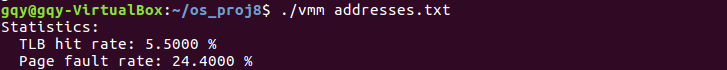
\includegraphics{vmm256}
		\caption{vmm测试(FRAME NUM=256)} \label{vmm测试(FRAME NUM=256)}
\end{figure}
\item[$\bullet$]vmm测试(FRAME NUM=128) (图 \ref{vmm测试(FRAME NUM=128)})
\begin{figure}[htbp]
		\centering
		
\includegraphics{vmm128}
		\caption{vmm测试(FRAME NUM=128)} \label{vmm测试(FRAME NUM=128)}
\end{figure}

测试指令如下
\begin{lstlisting}[language={[ANSI]C}]
make
./vmm addresses.txt
\end{lstlisting}
首先用Makefile文件编译,生成可执行文件vmm,然后对提供的addresses.txt执行,输出结果在文件answer.txt中,与提供的源文件correct.txt可以比较读取数据正确性,执行完成后打印了TLB命中率以及缺页率。图 \ref{vmm测试(FRAME NUM=256)}为设置物理内存帧数为256的测试结果,图 \ref{vmm测试(FRAME NUM=128)}为设置物理内存帧数为128的测试结果,两次测试的输出文件answer.txt与correct.txt对比都正确。
\end{itemize}
\section{Conclusion}

\subsection{问题与解决方案}
本次project8设计的虚拟内存管理器难度稍大,需要对物理内存,页表,TLB在根据地址读取信息的运行流程有比较透彻的理解,并且由于不同模块之间的相互作用,要设计高效且清晰的程序架构有较大的思考量。最开始我对于整个project的设计并没有什么头绪,几次翻阅书本并在头脑中不断复现整个虚拟内存工作流程后慢慢将整个工作分解为一个个函数,然后将其一个个实现出来,其中LRU置换策略的实现是一个难点,实现的过程中也出现了一些错误,仔细思考并调试后最后成功实现了。

\subsection{实验心得}
本次project8是对虚拟内存部分知识一次比较透彻的应用,在设计虚拟内存管理器的同时也帮助我对所学知识有了更深入的理解,而且本次project的架构根据虚拟内存原理而设计,函数相较于之前多且复杂,需要保持清醒的头脑,在程序出错的时候耐心寻找错误来源,也使编程能力有较大的提升。另外本次project也是操作系统课程设计的最后一个project,虽然在完成课程设计的时候会不断遇到一些问题,但最终都顺利实现了所有的项目内容,将理论知识和实践很好地结合在一起,总体来说让我受益匪浅。最后再一次感谢吴老师与助教们的悉心指导!




%----------------------------------------------------------------------------------------


\end{document}